\documentclass[10pt, a4paper]{article}
\usepackage{graphicx}
\usepackage{enumitem}
\usepackage{multicol}
\usepackage{setspace}
\usepackage[utf8]{inputenc}
\usepackage[T2A]{fontenc}
\usepackage[russian]{babel}
\usepackage{float}
\usepackage[nottoc]{tocbibind}
\usepackage[left=2.39cm,right=2.39cm,
    top=2.5cm,bottom=2.5cm]{geometry}
\newcommand{\RomanNumeralCaps}[1]{\MakeUppercase{\romannumeral#1}}

\begin{document}
\setcounter{figure}{9}
\setcounter{page}{228}
\setlist[itemize]{noitemsep, topsep=0pt}
\begin{multicols}{2}
\begin{figure}[H]
    \centering
   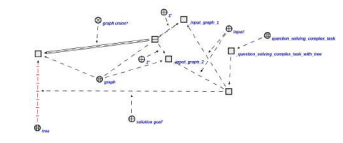
\includegraphics[width=\linewidth]{1screen.png}
    \caption{Task template}
\end{figure}
\vspace{4mm}
\begin{figure}[H]
    \centering
    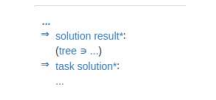
\includegraphics[width=0.4\textwidth]{2screen.png}
    \caption{Result of problem \label{11}}
\end{figure}
\vspace{9mm}
\par The result is shown in the figure \ref{11}. First the \textit{sc-agent of task specification generation by template} created a specification of a task and then it called \textit{sc-agent of solving a complex problem} which solved the problem because the \textit{knowledge base} had the statement that \textit{the tree is a connected acyclic graph}, the \textit{problem solver} knows how to determine whether the graph is connected or not, whether the graph is acyclic or has cycle and the \textit{problem solver} knows how to find the union of two graphs.
\begin{center}
   \RomanNumeralCaps{7.} Conclusion
\end{center}
\par Discrete mathematics is applied in various fields including logistics, geographical information systems, computer science, modeling of physical and mathematical phenomena, as well as sociology, biology, chemistry and economics, among others. Therefore, the development of an \textit{intelligent system} to solve problems directly or indirectly related to discrete mathematics is of great relevance and importance in modern society.\par Based on this work, the main components of \textit{intelligent tutoring systems for discrete mathematics} such as \textit{knowledge base},\textit{ problem solver} and \textit{user interface} have been identified and described. In addition to this, the requirements that all the components of the \textit{intelligent tutoring systems} should follow and their functions were also identified.\par Based on all the above, a prototype of \textit{intelligent tutoring systems for discrete mathematics} has been developed. However, this is only the beginning, and options for further development include the implementation of user tutoring and a personalized learning approach. 
\begin{center}
    Acknowledgment
\end{center}
\par The authors would like to thank the research groups of the Department of Intelligent Information Technologies of the Belarusian State University of Informatics and Radioelectronics
\begin{thebibliography}{196}
\setlength{\parskip}{0pt}
\setlength{\itemsep}{0pt}
\scriptsize
\bibitem  A. Liliya, “Social technologies and processes,” \textit{International scientific journal "BULLETIN OF SCIENCE" No. 1}, pp. 149–155, 2018.
\bibitem (2024, March) Wolfram|Alpha. [Online]. Available: https://www.wolframalpha.com/
\bibitem (2024, March) ALEKS - Assessment and LEarning in Knowledge Spaces. [Online]. Available: https://www.aleks.com/
\bibitem(2024, March) The WeBWorK Project. [Online]. Available: https://openwebwork.org/
\bibitem(2024, March) Maple T.A. [Online]. Available: https://www. maplesoft.com/
\bibitem V. Golenkov, N. Gulyakina, I. Davydenko, and D. Shunkevich, “Semanticheskie tekhnologii proektirovaniya intellektual’nyh sistem i semanticheskie associativnye komp’yutery [Semantic technologies of intelligent systems design and semantic associative computers],” \textit{Otkrytye semanticheskie tekhnologii proektirovaniya intellektual’nykh system [Open semantic technologies for intelligent systems]}, pp. 42–50, 2019, (In Russ.).
\bibitem V. V. Golenkov and N. A. Gulyakina, “Graphodynamic models of parallel knowledge processing: principles of construction, implementation and design,” \textit{Otkrytye semanticheskie tekhnologii proektirovaniya intellektual’nykh system [Open semantic technologies for intelligent systems]}, pp. 23–52, 2012.
\bibitem K. Bantsevich, “Structure of knowledge bases of next-generation intelligent computer systems: a hierarchical system of subject domains and their corresponding ontologies,”\textit{ Otkrytye semanticheskie tekhnologii proektirovaniya intellektual’nykh system [Open semantic technologies for intelligent systems]}, pp. 87–98, 2022.
\bibitem D. Shunkevich, “Agentno-orientirovannye reshateli zadach intellektual’nyh sistem [Agent-oriented models, method and tools of compatible problem solvers development for intelligent systems],” \textit{Otkrytye semanticheskie tekhnologii proektirovaniya intellektual’nykh system [Open semantic technologies for intelligent systems]}, pp. 119–132, 2018.
\bibitem A. S. Sharapov, “Designing knowledge bases of intelligent learning systems based on ostis technology,” \textit{A young scientist},
pp. 17–19, 2023. [Online]. Available: https://moluch.ru/archive/ 478/105252/
\bibitem W. G. Griswold, M. Shonle, K. Sullivan, Y. Song, N. Tewari, Y. Cai, and H. Rajan, “Modular software design with crosscutting interfaces,” \textit{IEEE software}, vol. 23, no. 1, pp. 51–60, 2006.
\bibitem   V. V. Golenkov, N. A. Gulyakina, D. G. Kolb, “Intelligent user interface,” pp. 35–36, 2013. [Online]. Available: https://libeldoc.bsuir.by/bitstream/123456789/998/2/\\Golenko\_Int.pdf
\end{thebibliography}
\begin{center}
    \textbf{ИНТЕЛЛЕКТУАЛЬНАЯ ОБУЧАЮЩАЯ СИСТЕМА ПО ДИСКРЕТНОЙ МАТЕМАТИКЕ}
\end{center}
\begin{center}
    Шурмель К. А., Шарапов А. С.,\\ Самохвал Е. С., Тищенко В. Н.
\end{center}
\par В статье представлена модель интеллектуальной обучающей системы по дискретной математике. Модель такой системы использует методы и средства, рассчитанные на построение интеллектуальных обучающих систем по любой дисциплине и простую интеграцию новых дисциплин в существующую обучающую систему.
\flushright Received 01.04.2024
\end{multicols}
\newpage
\section*{\huge Methods and Means of Constructing Plans for Solving Problems in Intelligent Systems on the Example of an Intelligent System on Geometry}
\vspace{2mm}
\begin{center}
     Natallia Malinovskaya and Anna Makarenko\\
    \textit{ Belarusian State University of\\ Informatics and Radioelectronics}
     \\ Minsk, Belarus\\
 Email: natasha.malinovskaya.9843@gmail.com, anna.makarenko1517@gmail.com
\end{center}
\vspace{2pt}
\begin{multicols}{2}
\textbf{\textit{Abstract}—In this paper we propose an approach to the development of methods and tools for constructing plans for solving problems in intelligent systems on the example of an intelligent system for geometry. The described approach is aimed at improving the accuracy of answers due to the possibility of decomposition of problems into simpler ones, and also aims to overcome the shortcomings of modern intelligent systems. An intelligent system realizing the proposed approach is described.]}
 \par \textbf{\textit{Keywords}—problem solving, knowledge, knowledge base, intelligent systems.}
 \begin{center}
    \RomanNumeralCaps{1.}  Introduction
 \end{center}
  \par Nowadays, the use of intelligent systems in various fields is becoming relevant. However, the quality of ISs is largely determined by its answers and the ability to solve complex problems, which is why it is necessary that its answers are as accurate and reliable as possible. In order to increase the accuracy of answers it is necessary to be able to decompose problems into simpler ones, in turn, the automation of this process will allow the IS to solve not only simple problems, but also complex, non trivial ones. The relevance of systems that have the ability not only to perform the above functions, but also have the ability to partially satisfy the human need for quick answers, allowing you to automate some of the routine actions.
\par Problem solver is one of the key components of ISs, allowing them to solve a wide range of problems. Unlike other modern software systems, the peculiarity of problem solvers in ISs is the necessity to solve problems in conditions when the necessary information for their solution is not explicitly localized in the knowledge base of the IS and must be found in the process of problem solving on the basis of certain criteria.
\par The composition of the problem solver in each particular system depends on its target, classes of solved problems, subject area and other factors. In general, a problem solver provides the ability to solve problems related both to the core functionality of the system and to ensure its efficient operation and development automation. A problem solver that performs all these functions is called a unified problem solver for a given IS.
\par Expanding the areas of application of ISs requires their ability to solve complex problems, which involve the joint use of different models of knowledge representation and problem solving models. In addition, solving complex problems involves the use of shared information resources, such as a knowledge base, by different components of the solver that specialize in solving different subproblems. Since a complex problem solver integrates different problem solving models, it is called a hybrid problem solver.
\par Examples of complex problems are:
\vspace{1pt}
\begin{itemize}
    \item problems related to understanding natural language texts (both printed and handwritten), understanding speech messages and images. In each of these cases it is required to perform syntactic analysis of the processed file or signal, remove insignificant fragments, classify significant fragments, relate them to concepts known to the system, etc.;
    \item automation of adaptive learning for schoolchildren and students, which implies that the system is capable of autonomously solving various problems from a certain subject area, as well as managing the learning process, generating tasks for students and controlling their independent fulfillment by the student;
    \item the problems of planning the behavior of intelligent robots, which involve both understanding a variety of external information and making various decisions using both credible methods and methods that rely on probabilistic estimates and plausible assumptions;
    \item problems related to complex and flexible automation of various enterprises.
    \item etc.
\end{itemize}
\vspace{4pt}
\par The use of different problem solving models within an IS implies decomposition of a complex problem into
\newpage
\noindent subproblems that can be solved using one of the known IS problem solving models. Due to the combination of different problem solving models, the set of problems solved by the hybrid solver will be much wider than the combination of sets of problems solved separately by all problem solvers included in its composition [1].
\par The existing variety of approaches to problem solving in computer systems can be divided into two classes:
\begin{itemize}[itemsep=0pt]
\setlength{\baselineskip}{0.87\baselineskip}
    \item
     problem solving using stored programs. In this case,
 it is assumed that the system has a program for
 solving a problem of a given class in advance,
 and the solution is reduced to searching for such a
 program and interpreting it on the given input data.
 The systems oriented on such approach to problem
 solving include systems using:
 \begin{itemize}
     \item [-]programs written in both imperative and declarative programming languages, including logical and functional programming [2];
     \item [-]genetic algorithm implementations [3], [4];
     \item [-]neural network models of knowledge processing
 [5], [6], [7].
 \end{itemize}
  It should be noted that even in the case of using a stored program, the solution of the problem is not always trivial, because, first, it is required to find such a stored program on the basis of some specification, and second, to provide its interpretation;
    \item solving problems in conditions where the solution
 program is not known.
\end{itemize}
 \noindent In this case, it is assumed that the system does not necessarily contain a ready-made solution program for the class of problems to which some formulated problem to be solved belongs. In this connection, it is necessary to apply additional methods of searching for ways to solve the problem, which are not designed for any narrow class of problems (e.g., splitting the problem into subproblems, methods of searching for solutions in depth and width, method of random solution search and trial-and-error method, etc.), as well as various models of logical inference (classical deductive, [8], inductive [9], [10], abductive [8]; models based on fuzzy logics [11], [12], [13], the logic of default [14], temporal logic [15], and many others).
\par For example, currently one of the most popular approaches to text generation for natural language problems is the use of \textit{large language models} [16], which are models consisting of neural networks with many parameters trained on a large amount of unlabeled text, but these models have a number of disadvantages, partial solution of which can be prevented by integration of such systems with knowledge bases [17], but this approach is not able to solve all the disadvantages of large language models in solving complex problems.
 \par Thus, although there have been significant advances in the development of problem solvers for ISs, there are still outstanding challenges related to provisioning:
 \begin{itemize}
 \setlength{\baselineskip}{0.9\baselineskip}
     \item  compatibility of different private problem solvers, i.e. the possibility of their coordinated use in solving the same complex problem;
     \item possibilities to modify the hybrid solver without significant additional costs in the process of operation of the IS. This includes expanding the number of used problem solving models without restrictions on their type. This requirement is due to the fact that when solving a complex problem, it may be unknown what specific problem-solving models and types of knowledge will be needed.
 \end{itemize}
\par The modern development of \textit{artificial intelligence} is moving towards the creation of intelligent computer systems of a new generation [18]. These systems are capable not only of solving problems from various fields of knowledge, but also of explaining their solutions. However, the disadvantages described above do not allow such systems to be built solely on the basis of existing solutions. Instead, new-generation ISs are built on a unified knowledge base that integrates problems, subject domains, and methods of their solution. Thus, we conclude that the use of modern solutions such as neural networks, models using specialized software interfaces between different system components, large language models can and should become a powerful tool for solving problems of ISs [19], but they cannot completely replace these systems [20].
\par  That is, despite the fact that currently there is a large number of problem-solving models, many of which are implemented and successfully used in practice in various systems, the problem of low consistency of the principles underlying the implementation of such models and the lack of a single unified framework for the implementation and integration of different models remains relevant, which leads to the fact that:
\begin{itemize}
\setlength{\baselineskip}{0.9\baselineskip}
    \item  it is difficult to simultaneously use different models of problem solving within one system when solving the same complex problem;
    \item  it is practically impossible to use technical solutions realized in one system in other systems;
    \item  in fact, there are no complex methods and tools for building problem solvers, which would provide the possibility of designing, realizing and debugging solvers of different kinds.
    \end{itemize}
    \par Therefore, the ability of an IS to independently solve non-trivial problems will expand the possible functionality of the IS, detail and improve the accuracy of its answers.
    \par The purpose of this study is to refine the ontologies of actions and problems, to develop a collective of agents that allows to divide the problem into subproblems, as well as to develop a methodology for the application of the obtained subsystem in specific application systems on the example of an IS for geometry.
\end{multicols}
\end{document}